\documentclass[1p]{elsarticle_modified}
%\bibliographystyle{elsarticle-num}

%\usepackage[colorlinks]{hyperref}
%\usepackage{abbrmath_seonhwa} %\Abb, \Ascr, \Acal ,\Abf, \Afrak
\usepackage{amsfonts}
\usepackage{amssymb}
\usepackage{amsmath}
\usepackage{amsthm}
\usepackage{scalefnt}
\usepackage{amsbsy}
\usepackage{kotex}
\usepackage{caption}
\usepackage{subfig}
\usepackage{color}
\usepackage{graphicx}
\usepackage{xcolor} %% white, black, red, green, blue, cyan, magenta, yellow
\usepackage{float}
\usepackage{setspace}
\usepackage{hyperref}

\usepackage{tikz}
\usetikzlibrary{arrows}

\usepackage{multirow}
\usepackage{array} % fixed length table
\usepackage{hhline}

%%%%%%%%%%%%%%%%%%%%%
\makeatletter
\renewcommand*\env@matrix[1][\arraystretch]{%
	\edef\arraystretch{#1}%
	\hskip -\arraycolsep
	\let\@ifnextchar\new@ifnextchar
	\array{*\c@MaxMatrixCols c}}
\makeatother %https://tex.stackexchange.com/questions/14071/how-can-i-increase-the-line-spacing-in-a-matrix
%%%%%%%%%%%%%%%

\usepackage[normalem]{ulem}

\newcommand{\msout}[1]{\ifmmode\text{\sout{\ensuremath{#1}}}\else\sout{#1}\fi}
%SOURCE: \msout is \stkout macro in https://tex.stackexchange.com/questions/20609/strikeout-in-math-mode

\newcommand{\cancel}[1]{
	\ifmmode
	{\color{red}\msout{#1}}
	\else
	{\color{red}\sout{#1}}
	\fi
}

\newcommand{\add}[1]{
	{\color{blue}\uwave{#1}}
}

\newcommand{\replace}[2]{
	\ifmmode
	{\color{red}\msout{#1}}{\color{blue}\uwave{#2}}
	\else
	{\color{red}\sout{#1}}{\color{blue}\uwave{#2}}
	\fi
}

\newcommand{\Sol}{\mathcal{S}} %segment
\newcommand{\D}{D} %diagram
\newcommand{\A}{\mathcal{A}} %arc


%%%%%%%%%%%%%%%%%%%%%%%%%%%%%5 test

\def\sl{\operatorname{\textup{SL}}(2,\Cbb)}
\def\psl{\operatorname{\textup{PSL}}(2,\Cbb)}
\def\quan{\mkern 1mu \triangleright \mkern 1mu}

\theoremstyle{definition}
\newtheorem{thm}{Theorem}[section]
\newtheorem{prop}[thm]{Proposition}
\newtheorem{lem}[thm]{Lemma}
\newtheorem{ques}[thm]{Question}
\newtheorem{cor}[thm]{Corollary}
\newtheorem{defn}[thm]{Definition}
\newtheorem{exam}[thm]{Example}
\newtheorem{rmk}[thm]{Remark}
\newtheorem{alg}[thm]{Algorithm}

\newcommand{\I}{\sqrt{-1}}
\begin{document}

%\begin{frontmatter}
%
%\title{Boundary parabolic representations of knots up to 8 crossings}
%
%%% Group authors per affiliation:
%\author{Yunhi Cho} 
%\address{Department of Mathematics, University of Seoul, Seoul, Korea}
%\ead{yhcho@uos.ac.kr}
%
%
%\author{Seonhwa Kim} %\fnref{s_kim}}
%\address{Center for Geometry and Physics, Institute for Basic Science, Pohang, 37673, Korea}
%\ead{ryeona17@ibs.re.kr}
%
%\author{Hyuk Kim}
%\address{Department of Mathematical Sciences, Seoul National University, Seoul 08826, Korea}
%\ead{hyukkim@snu.ac.kr}
%
%\author{Seokbeom Yoon}
%\address{Department of Mathematical Sciences, Seoul National University, Seoul, 08826,  Korea}
%\ead{sbyoon15@snu.ac.kr}
%
%\begin{abstract}
%We find all boundary parabolic representation of knots up to 8 crossings.
%
%\end{abstract}
%\begin{keyword}
%    \MSC[2010] 57M25 
%\end{keyword}
%
%\end{frontmatter}

%\linenumbers
%\tableofcontents
%
\newcommand\colored[1]{\textcolor{white}{\rule[-0.35ex]{0.8em}{1.4ex}}\kern-0.8em\color{red} #1}%
%\newcommand\colored[1]{\textcolor{white}{ #1}\kern-2.17ex	\textcolor{white}{ #1}\kern-1.81ex	\textcolor{white}{ #1}\kern-2.15ex\color{red}#1	}

{\Large $\underline{12n_{0265}~(K12n_{0265})}$}

\setlength{\tabcolsep}{10pt}
\renewcommand{\arraystretch}{1.6}
\vspace{1cm}\begin{tabular}{m{100pt}>{\centering\arraybackslash}m{274pt}}
\multirow{5}{120pt}{
	\centering
	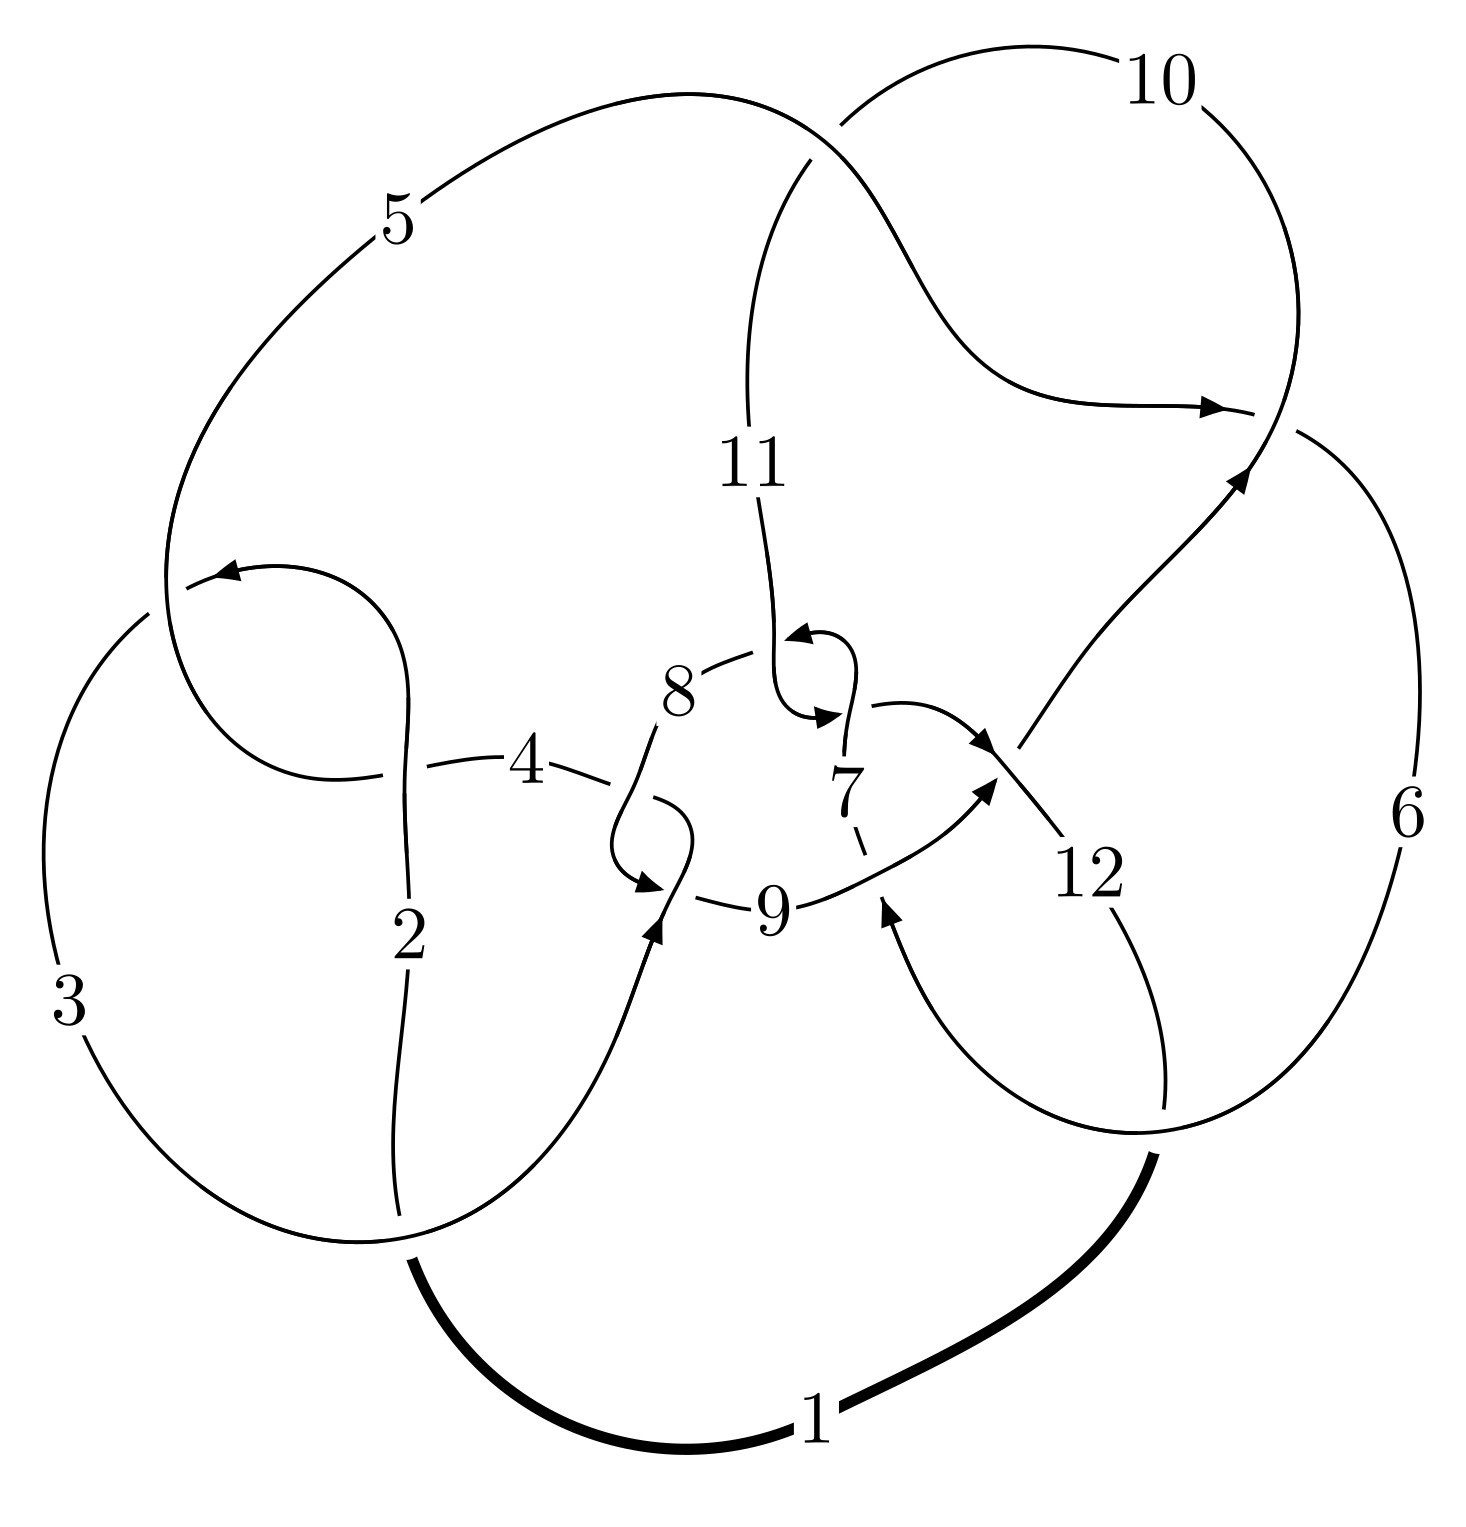
\includegraphics[width=112pt]{../../../GIT/diagram.site/Diagrams/png/2354_12n_0265.png}\\
\ \ \ A knot diagram\footnotemark}&
\allowdisplaybreaks
\textbf{Linearized knot diagam} \\
\cline{2-2}
 &
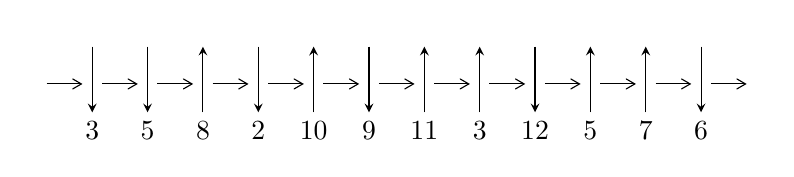
\begin{tikzpicture}[x=20pt, y=17pt]
	% nodes
	\node (C0) at (0, 0) {};
	\node (C1) at (1, 0) {};
	\node (C1U) at (1, +1) {};
	\node (C1D) at (1, -1) {3};

	\node (C2) at (2, 0) {};
	\node (C2U) at (2, +1) {};
	\node (C2D) at (2, -1) {5};

	\node (C3) at (3, 0) {};
	\node (C3U) at (3, +1) {};
	\node (C3D) at (3, -1) {8};

	\node (C4) at (4, 0) {};
	\node (C4U) at (4, +1) {};
	\node (C4D) at (4, -1) {2};

	\node (C5) at (5, 0) {};
	\node (C5U) at (5, +1) {};
	\node (C5D) at (5, -1) {10};

	\node (C6) at (6, 0) {};
	\node (C6U) at (6, +1) {};
	\node (C6D) at (6, -1) {9};

	\node (C7) at (7, 0) {};
	\node (C7U) at (7, +1) {};
	\node (C7D) at (7, -1) {11};

	\node (C8) at (8, 0) {};
	\node (C8U) at (8, +1) {};
	\node (C8D) at (8, -1) {3};

	\node (C9) at (9, 0) {};
	\node (C9U) at (9, +1) {};
	\node (C9D) at (9, -1) {12};

	\node (C10) at (10, 0) {};
	\node (C10U) at (10, +1) {};
	\node (C10D) at (10, -1) {5};

	\node (C11) at (11, 0) {};
	\node (C11U) at (11, +1) {};
	\node (C11D) at (11, -1) {7};

	\node (C12) at (12, 0) {};
	\node (C12U) at (12, +1) {};
	\node (C12D) at (12, -1) {6};
	\node (C13) at (13, 0) {};

	% arrows
	\draw[->,>={angle 60}]
	(C0) edge (C1) (C1) edge (C2) (C2) edge (C3) (C3) edge (C4) (C4) edge (C5) (C5) edge (C6) (C6) edge (C7) (C7) edge (C8) (C8) edge (C9) (C9) edge (C10) (C10) edge (C11) (C11) edge (C12) (C12) edge (C13) ;	\draw[->,>=stealth]
	(C1U) edge (C1D) (C2U) edge (C2D) (C3D) edge (C3U) (C4U) edge (C4D) (C5D) edge (C5U) (C6U) edge (C6D) (C7D) edge (C7U) (C8D) edge (C8U) (C9U) edge (C9D) (C10D) edge (C10U) (C11D) edge (C11U) (C12U) edge (C12D) ;
	\end{tikzpicture} \\
\hhline{~~} \\& 
\textbf{Solving Sequence} \\ \cline{2-2} 
 &
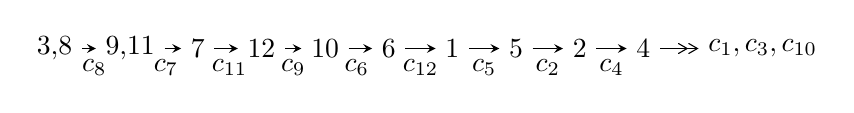
\begin{tikzpicture}[x=23pt, y=7pt]
	% node
	\node (A0) at (-1/8, 0) {3,8};
	\node (A1) at (17/16, 0) {9,11};
	\node (A2) at (17/8, 0) {7};
	\node (A3) at (25/8, 0) {12};
	\node (A4) at (33/8, 0) {10};
	\node (A5) at (41/8, 0) {6};
	\node (A6) at (49/8, 0) {1};
	\node (A7) at (57/8, 0) {5};
	\node (A8) at (65/8, 0) {2};
	\node (A9) at (73/8, 0) {4};
	\node (C1) at (1/2, -1) {$c_{8}$};
	\node (C2) at (13/8, -1) {$c_{7}$};
	\node (C3) at (21/8, -1) {$c_{11}$};
	\node (C4) at (29/8, -1) {$c_{9}$};
	\node (C5) at (37/8, -1) {$c_{6}$};
	\node (C6) at (45/8, -1) {$c_{12}$};
	\node (C7) at (53/8, -1) {$c_{5}$};
	\node (C8) at (61/8, -1) {$c_{2}$};
	\node (C9) at (69/8, -1) {$c_{4}$};
	\node (A10) at (11, 0) {$c_{1},c_{3},c_{10}$};

	% edge
	\draw[->,>=stealth]	
	(A0) edge (A1) (A1) edge (A2) (A2) edge (A3) (A3) edge (A4) (A4) edge (A5) (A5) edge (A6) (A6) edge (A7) (A7) edge (A8) (A8) edge (A9) ;
	\draw[->>,>={angle 60}]	
	(A9) edge (A10);
\end{tikzpicture} \\ 

\end{tabular} \\

\footnotetext{
The image of knot diagram is generated by the software ``\textbf{Draw programme}" developed by Andrew Bartholomew(\url{http://www.layer8.co.uk/maths/draw/index.htm\#Running-draw}), where we modified some parts for our purpose(\url{https://github.com/CATsTAILs/LinksPainter}).
}\phantom \\ \newline 
\centering \textbf{Ideals for irreducible components\footnotemark of $X_{\text{par}}$} 
 
\begin{align*}
I^u_{1}&=\langle 
2.44371\times10^{49} u^{24}-2.09348\times10^{50} u^{23}+\cdots+2.28036\times10^{53} b-8.49453\times10^{51},\\
\phantom{I^u_{1}}&\phantom{= \langle  }-3.67178\times10^{50} u^{24}+2.53945\times10^{51} u^{23}+\cdots+1.82429\times10^{54} a-1.58059\times10^{54},\\
\phantom{I^u_{1}}&\phantom{= \langle  }u^{25}-7 u^{24}+\cdots-768 u-1024\rangle \\
I^u_{2}&=\langle 
1765 a^5 u^4-1502 a^4 u^4+\cdots+17362 a-4182,\;-2 a^5 u^4+22 a^4 u^4+\cdots-398 a-265,\\
\phantom{I^u_{2}}&\phantom{= \langle  }u^5+u^4+5 u^3+u^2+2 u-2\rangle \\
I^u_{3}&=\langle 
94430 u^{13}-176465 u^{12}+\cdots+3057583 b-933114,\\
\phantom{I^u_{3}}&\phantom{= \langle  }11442968 u^{13}-3792535 u^{12}+\cdots+3057583 a+15949942,\\
\phantom{I^u_{3}}&\phantom{= \langle  }u^{14}+3 u^{12}+3 u^{11}-5 u^{10}-4 u^9-11 u^8-8 u^7+12 u^6-8 u^5+20 u^4+6 u^2+u+1\rangle \\
\\
I^v_{1}&=\langle 
a,\;8 v^3-12 v^2+b+10 v-3,\;8 v^4-12 v^3+12 v^2-5 v+1\rangle \\
I^v_{2}&=\langle 
a,\;b^6- b^5+2 b^4-2 b^3+2 b^2-2 b+1,\;v+1\rangle \\
\end{align*}
\raggedright * 5 irreducible components of $\dim_{\mathbb{C}}=0$, with total 79 representations.\\
\footnotetext{All coefficients of polynomials are rational numbers. But the coefficients are sometimes approximated in decimal forms when there is not enough margin.}
\newpage
\renewcommand{\arraystretch}{1}
\centering \section*{I. $I^u_{1}= \langle 2.44\times10^{49} u^{24}-2.09\times10^{50} u^{23}+\cdots+2.28\times10^{53} b-8.49\times10^{51},\;-3.67\times10^{50} u^{24}+2.54\times10^{51} u^{23}+\cdots+1.82\times10^{54} a-1.58\times10^{54},\;u^{25}-7 u^{24}+\cdots-768 u-1024 \rangle$}
\flushleft \textbf{(i) Arc colorings}\\
\begin{tabular}{m{7pt} m{180pt} m{7pt} m{180pt} }
\flushright $a_{3}=$&$\begin{pmatrix}0\\u\end{pmatrix}$ \\
\flushright $a_{8}=$&$\begin{pmatrix}1\\0\end{pmatrix}$ \\
\flushright $a_{9}=$&$\begin{pmatrix}1\\- u^2\end{pmatrix}$ \\
\flushright $a_{11}=$&$\begin{pmatrix}0.000201272 u^{24}-0.00139202 u^{23}+\cdots+0.373312 u+0.866413\\-0.000107163 u^{24}+0.000918045 u^{23}+\cdots+0.329212 u+0.0372508\end{pmatrix}$ \\
\flushright $a_{7}=$&$\begin{pmatrix}0.000229394 u^{24}-0.00150305 u^{23}+\cdots+0.0571684 u+0.797253\\0.000436197 u^{24}-0.00314869 u^{23}+\cdots+0.195357 u-0.517398\end{pmatrix}$ \\
\flushright $a_{12}=$&$\begin{pmatrix}0.000142173 u^{24}-0.000866042 u^{23}+\cdots+0.288083 u+0.794249\\0.0000403596 u^{24}-0.000408965 u^{23}+\cdots+0.135333 u-0.227239\end{pmatrix}$ \\
\flushright $a_{10}=$&$\begin{pmatrix}0.000280396 u^{24}-0.00189155 u^{23}+\cdots+0.798559 u+1.20818\\-0.000127304 u^{24}+0.00120796 u^{23}+\cdots+0.0853997 u+0.470901\end{pmatrix}$ \\
\flushright $a_{6}=$&$\begin{pmatrix}0.000729995 u^{24}-0.00506873 u^{23}+\cdots+0.566298 u+0.385020\\0.000193200 u^{24}-0.00159495 u^{23}+\cdots-0.270058 u-0.454462\end{pmatrix}$ \\
\flushright $a_{1}=$&$\begin{pmatrix}0.000602735 u^{24}-0.00397878 u^{23}+\cdots+0.982564 u+0.885973\\-0.000178179 u^{24}+0.00103362 u^{23}+\cdots-0.219803 u-0.141734\end{pmatrix}$ \\
\flushright $a_{5}=$&$\begin{pmatrix}0.000548097 u^{24}-0.00349779 u^{23}+\cdots+0.400564 u+0.781569\\-0.0000546374 u^{24}+0.000480983 u^{23}+\cdots-0.582000 u-0.104403\end{pmatrix}$ \\
\flushright $a_{2}=$&$\begin{pmatrix}0.000602735 u^{24}-0.00397878 u^{23}+\cdots+0.982564 u+0.885973\\0.0000546374 u^{24}-0.000480983 u^{23}+\cdots+0.582000 u+0.104403\end{pmatrix}$ \\
\flushright $a_{4}=$&$\begin{pmatrix}- u\\- u\end{pmatrix}$\\&\end{tabular}
\flushleft \textbf{(ii) Obstruction class $= -1$}\\~\\
\flushleft \textbf{(iii) Cusp Shapes $= -0.00281397 u^{24}+0.0194032 u^{23}+\cdots-9.17416 u+2.20110$}\\~\\
\newpage\renewcommand{\arraystretch}{1}
\flushleft \textbf{(iv) u-Polynomials at the component}\newline \\
\begin{tabular}{m{50pt}|m{274pt}}
Crossings & \hspace{64pt}u-Polynomials at each crossing \\
\hline $$\begin{aligned}c_{1}\end{aligned}$$&$\begin{aligned}
&u^{25}+25 u^{24}+\cdots-39680 u+4096
\end{aligned}$\\
\hline $$\begin{aligned}c_{2},c_{4}\end{aligned}$$&$\begin{aligned}
&u^{25}-5 u^{24}+\cdots-272 u+64
\end{aligned}$\\
\hline $$\begin{aligned}c_{3},c_{8}\end{aligned}$$&$\begin{aligned}
&u^{25}+7 u^{24}+\cdots-768 u+1024
\end{aligned}$\\
\hline $$\begin{aligned}c_{5},c_{7},c_{10}\\c_{11}\end{aligned}$$&$\begin{aligned}
&u^{25}+16 u^{23}+\cdots-4 u-1
\end{aligned}$\\
\hline $$\begin{aligned}c_{6},c_{12}\end{aligned}$$&$\begin{aligned}
&u^{25}- u^{24}+\cdots-3 u-1
\end{aligned}$\\
\hline $$\begin{aligned}c_{9}\end{aligned}$$&$\begin{aligned}
&u^{25}-17 u^{24}+\cdots+304 u-32
\end{aligned}$\\
\hline
\end{tabular}\\~\\
\newpage\renewcommand{\arraystretch}{1}
\flushleft \textbf{(v) Riley Polynomials at the component}\newline \\
\begin{tabular}{m{50pt}|m{274pt}}
Crossings & \hspace{64pt}Riley Polynomials at each crossing \\
\hline $$\begin{aligned}c_{1}\end{aligned}$$&$\begin{aligned}
&y^{25}-45 y^{24}+\cdots+260374528 y-16777216
\end{aligned}$\\
\hline $$\begin{aligned}c_{2},c_{4}\end{aligned}$$&$\begin{aligned}
&y^{25}-25 y^{24}+\cdots-39680 y-4096
\end{aligned}$\\
\hline $$\begin{aligned}c_{3},c_{8}\end{aligned}$$&$\begin{aligned}
&y^{25}+15 y^{24}+\cdots+3473408 y-1048576
\end{aligned}$\\
\hline $$\begin{aligned}c_{5},c_{7},c_{10}\\c_{11}\end{aligned}$$&$\begin{aligned}
&y^{25}+32 y^{24}+\cdots+6 y-1
\end{aligned}$\\
\hline $$\begin{aligned}c_{6},c_{12}\end{aligned}$$&$\begin{aligned}
&y^{25}-19 y^{24}+\cdots-27 y-1
\end{aligned}$\\
\hline $$\begin{aligned}c_{9}\end{aligned}$$&$\begin{aligned}
&y^{25}+3 y^{24}+\cdots+6912 y-1024
\end{aligned}$\\
\hline
\end{tabular}\\~\\
\newpage\flushleft \textbf{(vi) Complex Volumes and Cusp Shapes}
$$\begin{array}{c|c|c}  
\text{Solutions to }I^u_{1}& \I (\text{vol} + \sqrt{-1}CS) & \text{Cusp shape}\\
 \hline 
\begin{aligned}
u &= -0.239284 + 0.960930 I \\
a &= \phantom{-}0.533027 - 0.309402 I \\
b &= \phantom{-}0.493247 + 0.016890 I\end{aligned}
 & -0.98698 - 2.00436 I & \phantom{-}0.63223 + 3.08678 I \\ \hline\begin{aligned}
u &= -0.239284 - 0.960930 I \\
a &= \phantom{-}0.533027 + 0.309402 I \\
b &= \phantom{-}0.493247 - 0.016890 I\end{aligned}
 & -0.98698 + 2.00436 I & \phantom{-}0.63223 - 3.08678 I \\ \hline\begin{aligned}
u &= \phantom{-}0.966851\phantom{ +0.000000I} \\
a &= \phantom{-}0.382684\phantom{ +0.000000I} \\
b &= -0.452501\phantom{ +0.000000I}\end{aligned}
 & -3.00634\phantom{ +0.000000I} & -1.07640\phantom{ +0.000000I} \\ \hline\begin{aligned}
u &= \phantom{-}1.116350 + 0.182242 I \\
a &= \phantom{-}0.381438 - 0.739225 I \\
b &= -0.224461 - 0.800052 I\end{aligned}
 & \phantom{-}0.48422 + 3.81324 I & \phantom{-}7.26566 - 4.06355 I \\ \hline\begin{aligned}
u &= \phantom{-}1.116350 - 0.182242 I \\
a &= \phantom{-}0.381438 + 0.739225 I \\
b &= -0.224461 + 0.800052 I\end{aligned}
 & \phantom{-}0.48422 - 3.81324 I & \phantom{-}7.26566 + 4.06355 I \\ \hline\begin{aligned}
u &= -0.697727 + 0.198752 I \\
a &= -0.164828 + 0.368624 I \\
b &= \phantom{-}0.521134 + 1.221040 I\end{aligned}
 & -3.96011 + 7.15054 I & \phantom{-}0.209463 - 0.912602 I \\ \hline\begin{aligned}
u &= -0.697727 - 0.198752 I \\
a &= -0.164828 - 0.368624 I \\
b &= \phantom{-}0.521134 - 1.221040 I\end{aligned}
 & -3.96011 - 7.15054 I & \phantom{-}0.209463 + 0.912602 I \\ \hline\begin{aligned}
u &= \phantom{-}0.407422 + 1.271680 I \\
a &= \phantom{-}0.154193 + 0.247049 I \\
b &= \phantom{-}0.470617 + 0.132952 I\end{aligned}
 & -7.17114 + 4.86761 I & \phantom{-}3.67428 + 1.38704 I \\ \hline\begin{aligned}
u &= \phantom{-}0.407422 - 1.271680 I \\
a &= \phantom{-}0.154193 - 0.247049 I \\
b &= \phantom{-}0.470617 - 0.132952 I\end{aligned}
 & -7.17114 - 4.86761 I & \phantom{-}3.67428 - 1.38704 I \\ \hline\begin{aligned}
u &= \phantom{-}0.356543 + 0.532418 I \\
a &= \phantom{-}1.40268 - 0.66297 I \\
b &= \phantom{-}0.145873 - 0.427689 I\end{aligned}
 & -1.84591 - 0.75519 I & -5.74786 - 0.43805 I\\
 \hline 
 \end{array}$$\newpage$$\begin{array}{c|c|c}  
\text{Solutions to }I^u_{1}& \I (\text{vol} + \sqrt{-1}CS) & \text{Cusp shape}\\
 \hline 
\begin{aligned}
u &= \phantom{-}0.356543 - 0.532418 I \\
a &= \phantom{-}1.40268 + 0.66297 I \\
b &= \phantom{-}0.145873 + 0.427689 I\end{aligned}
 & -1.84591 + 0.75519 I & -5.74786 + 0.43805 I \\ \hline\begin{aligned}
u &= -0.481170 + 0.308405 I \\
a &= \phantom{-}0.517741 + 0.397349 I \\
b &= -0.458678 + 0.410360 I\end{aligned}
 & \phantom{-}0.898356 - 0.808185 I & \phantom{-}6.63316 + 4.13450 I \\ \hline\begin{aligned}
u &= -0.481170 - 0.308405 I \\
a &= \phantom{-}0.517741 - 0.397349 I \\
b &= -0.458678 - 0.410360 I\end{aligned}
 & \phantom{-}0.898356 + 0.808185 I & \phantom{-}6.63316 - 4.13450 I \\ \hline\begin{aligned}
u &= -1.24876 + 0.83504 I \\
a &= \phantom{-}0.202515 - 0.510317 I \\
b &= -0.516721 - 1.100670 I\end{aligned}
 & -0.688755 - 0.842359 I & -3.27794 - 2.99522 I \\ \hline\begin{aligned}
u &= -1.24876 - 0.83504 I \\
a &= \phantom{-}0.202515 + 0.510317 I \\
b &= -0.516721 + 1.100670 I\end{aligned}
 & -0.688755 + 0.842359 I & -3.27794 + 2.99522 I \\ \hline\begin{aligned}
u &= -0.19971 + 2.12744 I \\
a &= \phantom{-}0.089187 + 1.142770 I \\
b &= -0.29018 + 1.74806 I\end{aligned}
 & -12.2506 - 8.8129 I & -5.58581 + 4.80434 I \\ \hline\begin{aligned}
u &= -0.19971 - 2.12744 I \\
a &= \phantom{-}0.089187 - 1.142770 I \\
b &= -0.29018 - 1.74806 I\end{aligned}
 & -12.2506 + 8.8129 I & -5.58581 - 4.80434 I \\ \hline\begin{aligned}
u &= \phantom{-}1.03266 + 1.89173 I \\
a &= \phantom{-}0.583269 - 0.980042 I \\
b &= -0.67321 - 1.74414 I\end{aligned}
 & \phantom{-}19.0826 + 15.6197 I & -5.76128 - 6.47974 I \\ \hline\begin{aligned}
u &= \phantom{-}1.03266 - 1.89173 I \\
a &= \phantom{-}0.583269 + 0.980042 I \\
b &= -0.67321 + 1.74414 I\end{aligned}
 & \phantom{-}19.0826 - 15.6197 I & -5.76128 + 6.47974 I \\ \hline\begin{aligned}
u &= -0.58061 + 2.17440 I \\
a &= -0.286368 - 1.009020 I \\
b &= \phantom{-}0.12493 - 1.68098 I\end{aligned}
 & -11.69760 + 0.19520 I & -6.36512 + 0. I\phantom{ +0.000000I}\\
 \hline 
 \end{array}$$\newpage$$\begin{array}{c|c|c}  
\text{Solutions to }I^u_{1}& \I (\text{vol} + \sqrt{-1}CS) & \text{Cusp shape}\\
 \hline 
\begin{aligned}
u &= -0.58061 - 2.17440 I \\
a &= -0.286368 + 1.009020 I \\
b &= \phantom{-}0.12493 + 1.68098 I\end{aligned}
 & -11.69760 - 0.19520 I & -6.36512 + 0. I\phantom{ +0.000000I} \\ \hline\begin{aligned}
u &= \phantom{-}1.23926 + 1.89887 I \\
a &= -0.567788 + 0.851816 I \\
b &= \phantom{-}0.55518 + 1.55240 I\end{aligned}
 & -19.1706 + 7.3377 I & -6.38194 - 3.47918 I \\ \hline\begin{aligned}
u &= \phantom{-}1.23926 - 1.89887 I \\
a &= -0.567788 - 0.851816 I \\
b &= \phantom{-}0.55518 - 1.55240 I\end{aligned}
 & -19.1706 - 7.3377 I & -6.38194 + 3.47918 I \\ \hline\begin{aligned}
u &= \phantom{-}2.31161 + 0.19224 I \\
a &= -0.036412 + 0.377901 I \\
b &= \phantom{-}0.07852 + 1.79165 I\end{aligned}
 & -14.6508 + 4.4763 I & -6.63166 - 2.50646 I \\ \hline\begin{aligned}
u &= \phantom{-}2.31161 - 0.19224 I \\
a &= -0.036412 - 0.377901 I \\
b &= \phantom{-}0.07852 - 1.79165 I\end{aligned}
 & -14.6508 - 4.4763 I & -6.63166 + 2.50646 I\\
 \hline 
 \end{array}$$\newpage\newpage\renewcommand{\arraystretch}{1}
\centering \section*{II. $I^u_{2}= \langle 1765 a^5 u^4-1502 a^4 u^4+\cdots+17362 a-4182,\;-2 a^5 u^4+22 a^4 u^4+\cdots-398 a-265,\;u^5+u^4+5 u^3+u^2+2 u-2 \rangle$}
\flushleft \textbf{(i) Arc colorings}\\
\begin{tabular}{m{7pt} m{180pt} m{7pt} m{180pt} }
\flushright $a_{3}=$&$\begin{pmatrix}0\\u\end{pmatrix}$ \\
\flushright $a_{8}=$&$\begin{pmatrix}1\\0\end{pmatrix}$ \\
\flushright $a_{9}=$&$\begin{pmatrix}1\\- u^2\end{pmatrix}$ \\
\flushright $a_{11}=$&$\begin{pmatrix}a\\-1.22230 a^{5} u^{4}+1.04017 a^{4} u^{4}+\cdots-12.0235 a+2.89612\end{pmatrix}$ \\
\flushright $a_{7}=$&$\begin{pmatrix}-0.407202 a^{5} u^{4}+1.61911 a^{4} u^{4}+\cdots-12.4986 a+10.4488\\1.02216 a^{5} u^{4}+0.364266 a^{4} u^{4}+\cdots+4.14958 a-2.79778\end{pmatrix}$ \\
\flushright $a_{12}=$&$\begin{pmatrix}-1.26593 a^{5} u^{4}+0.393352 a^{4} u^{4}+\cdots-13.1371 a+0.155125\\-1.72022 a^{5} u^{4}-3.92521 a^{4} u^{4}+\cdots+10.4017 a-6.69252\end{pmatrix}$ \\
\flushright $a_{10}=$&$\begin{pmatrix}0.0117729 a^{5} u^{4}-0.395429 a^{4} u^{4}+\cdots+4.60249 a-1.10665\\-1.61150 a^{5} u^{4}+0.450831 a^{4} u^{4}+\cdots-6.61773 a+1.48061\end{pmatrix}$ \\
\flushright $a_{6}=$&$\begin{pmatrix}-0.407202 a^{5} u^{4}+1.61911 a^{4} u^{4}+\cdots-12.4986 a+9.18560\\1.02216 a^{5} u^{4}+0.364266 a^{4} u^{4}+\cdots+4.14958 a-3.21884\end{pmatrix}$ \\
\flushright $a_{1}=$&$\begin{pmatrix}\frac{1}{4} u^4+\frac{1}{2} u^3+\cdots+\frac{1}{2} u-\frac{1}{2}\\\frac{1}{4} u^4+\frac{3}{2} u^3+\frac{7}{4} u^2+u-\frac{1}{2}\end{pmatrix}$ \\
\flushright $a_{5}=$&$\begin{pmatrix}\frac{1}{4} u^4+\frac{3}{4} u^2-\frac{1}{2} u-\frac{1}{2}\\-\frac{1}{2} u^3-\frac{1}{2} u^2- u\end{pmatrix}$ \\
\flushright $a_{2}=$&$\begin{pmatrix}\frac{1}{4} u^4+\frac{1}{2} u^3+\cdots+\frac{1}{2} u-\frac{1}{2}\\\frac{1}{2} u^3+\frac{1}{2} u^2+u\end{pmatrix}$ \\
\flushright $a_{4}=$&$\begin{pmatrix}- u\\- u\end{pmatrix}$\\&\end{tabular}
\flushleft \textbf{(ii) Obstruction class $= -1$}\\~\\
\flushleft \textbf{(iii) Cusp Shapes $= -\frac{588}{361} a^4 u^4+\frac{53}{19} u^4 a^3+\cdots+\frac{434}{19} a-\frac{9308}{361}$}\\~\\
\newpage\renewcommand{\arraystretch}{1}
\flushleft \textbf{(iv) u-Polynomials at the component}\newline \\
\begin{tabular}{m{50pt}|m{274pt}}
Crossings & \hspace{64pt}u-Polynomials at each crossing \\
\hline $$\begin{aligned}c_{1}\end{aligned}$$&$\begin{aligned}
&(u^5+8 u^4+22 u^3+25 u^2+15 u+1)^6
\end{aligned}$\\
\hline $$\begin{aligned}c_{2},c_{4}\end{aligned}$$&$\begin{aligned}
&(u^5-2 u^4-2 u^3+3 u^2+3 u-1)^6
\end{aligned}$\\
\hline $$\begin{aligned}c_{3},c_{8}\end{aligned}$$&$\begin{aligned}
&(u^5- u^4+5 u^3- u^2+2 u+2)^6
\end{aligned}$\\
\hline $$\begin{aligned}c_{5},c_{7},c_{10}\\c_{11}\end{aligned}$$&$\begin{aligned}
&u^{30}-2 u^{29}+\cdots+4896 u+1161
\end{aligned}$\\
\hline $$\begin{aligned}c_{6},c_{12}\end{aligned}$$&$\begin{aligned}
&u^{30}-6 u^{29}+\cdots-2892 u+367
\end{aligned}$\\
\hline $$\begin{aligned}c_{9}\end{aligned}$$&$\begin{aligned}
&(u^3+u^2-1)^{10}
\end{aligned}$\\
\hline
\end{tabular}\\~\\
\newpage\renewcommand{\arraystretch}{1}
\flushleft \textbf{(v) Riley Polynomials at the component}\newline \\
\begin{tabular}{m{50pt}|m{274pt}}
Crossings & \hspace{64pt}Riley Polynomials at each crossing \\
\hline $$\begin{aligned}c_{1}\end{aligned}$$&$\begin{aligned}
&(y^5-20 y^4+114 y^3+19 y^2+175 y-1)^6
\end{aligned}$\\
\hline $$\begin{aligned}c_{2},c_{4}\end{aligned}$$&$\begin{aligned}
&(y^5-8 y^4+22 y^3-25 y^2+15 y-1)^6
\end{aligned}$\\
\hline $$\begin{aligned}c_{3},c_{8}\end{aligned}$$&$\begin{aligned}
&(y^5+9 y^4+27 y^3+23 y^2+8 y-4)^6
\end{aligned}$\\
\hline $$\begin{aligned}c_{5},c_{7},c_{10}\\c_{11}\end{aligned}$$&$\begin{aligned}
&y^{30}+30 y^{29}+\cdots+10260108 y+1347921
\end{aligned}$\\
\hline $$\begin{aligned}c_{6},c_{12}\end{aligned}$$&$\begin{aligned}
&y^{30}-10 y^{29}+\cdots-2032180 y+134689
\end{aligned}$\\
\hline $$\begin{aligned}c_{9}\end{aligned}$$&$\begin{aligned}
&(y^3- y^2+2 y-1)^{10}
\end{aligned}$\\
\hline
\end{tabular}\\~\\
\newpage\flushleft \textbf{(vi) Complex Volumes and Cusp Shapes}
$$\begin{array}{c|c|c}  
\text{Solutions to }I^u_{2}& \I (\text{vol} + \sqrt{-1}CS) & \text{Cusp shape}\\
 \hline 
\begin{aligned}
u &= -0.375669 + 0.888717 I \\
a &= -0.218883 + 0.638145 I \\
b &= -0.936331 - 0.693043 I\end{aligned}
 & -3.76205 + 3.93704 I & -6.85572 - 5.02057 I \\ \hline\begin{aligned}
u &= -0.375669 + 0.888717 I \\
a &= -1.341030 + 0.088898 I \\
b &= \phantom{-}0.131979 + 0.509733 I\end{aligned}
 & -3.76205 - 1.71921 I & -6.85572 + 0.93832 I \\ \hline\begin{aligned}
u &= -0.375669 + 0.888717 I \\
a &= -1.69246 - 1.78412 I \\
b &= -0.22064 - 1.80276 I\end{aligned}
 & -7.89964 + 1.10891 I & -13.38499 - 2.04112 I \\ \hline\begin{aligned}
u &= -0.375669 + 0.888717 I \\
a &= \phantom{-}0.48486 + 2.82858 I \\
b &= \phantom{-}0.03993 + 1.45055 I\end{aligned}
 & -7.89964 + 1.10891 I & -13.38499 - 2.04112 I \\ \hline\begin{aligned}
u &= -0.375669 + 0.888717 I \\
a &= -1.51063 - 2.46477 I \\
b &= \phantom{-}0.607737 - 1.057200 I\end{aligned}
 & -3.76205 - 1.71921 I & -6.85572 + 0.93832 I \\ \hline\begin{aligned}
u &= -0.375669 + 0.888717 I \\
a &= \phantom{-}2.15895 + 2.52617 I \\
b &= \phantom{-}0.060199 + 0.974637 I\end{aligned}
 & -3.76205 + 3.93704 I & -6.85572 - 5.02057 I \\ \hline\begin{aligned}
u &= -0.375669 - 0.888717 I \\
a &= -0.218883 - 0.638145 I \\
b &= -0.936331 + 0.693043 I\end{aligned}
 & -3.76205 - 3.93704 I & -6.85572 + 5.02057 I \\ \hline\begin{aligned}
u &= -0.375669 - 0.888717 I \\
a &= -1.341030 - 0.088898 I \\
b &= \phantom{-}0.131979 - 0.509733 I\end{aligned}
 & -3.76205 + 1.71921 I & -6.85572 - 0.93832 I \\ \hline\begin{aligned}
u &= -0.375669 - 0.888717 I \\
a &= -1.69246 + 1.78412 I \\
b &= -0.22064 + 1.80276 I\end{aligned}
 & -7.89964 - 1.10891 I & -13.38499 + 2.04112 I \\ \hline\begin{aligned}
u &= -0.375669 - 0.888717 I \\
a &= \phantom{-}0.48486 - 2.82858 I \\
b &= \phantom{-}0.03993 - 1.45055 I\end{aligned}
 & -7.89964 - 1.10891 I & -13.38499 + 2.04112 I\\
 \hline 
 \end{array}$$\newpage$$\begin{array}{c|c|c}  
\text{Solutions to }I^u_{2}& \I (\text{vol} + \sqrt{-1}CS) & \text{Cusp shape}\\
 \hline 
\begin{aligned}
u &= -0.375669 - 0.888717 I \\
a &= -1.51063 + 2.46477 I \\
b &= \phantom{-}0.607737 + 1.057200 I\end{aligned}
 & -3.76205 + 1.71921 I & -6.85572 - 0.93832 I \\ \hline\begin{aligned}
u &= -0.375669 - 0.888717 I \\
a &= \phantom{-}2.15895 - 2.52617 I \\
b &= \phantom{-}0.060199 - 0.974637 I\end{aligned}
 & -3.76205 - 3.93704 I & -6.85572 + 5.02057 I \\ \hline\begin{aligned}
u &= \phantom{-}0.504107\phantom{ +0.000000I} \\
a &= \phantom{-}0.528054 + 0.820274 I \\
b &= \phantom{-}0.237566 - 1.254220 I\end{aligned}
 & -4.84461\phantom{ +0.000000I} & -2.07647 + 0. I\phantom{ +0.000000I} \\ \hline\begin{aligned}
u &= \phantom{-}0.504107\phantom{ +0.000000I} \\
a &= \phantom{-}0.528054 - 0.820274 I \\
b &= \phantom{-}0.237566 + 1.254220 I\end{aligned}
 & -4.84461\phantom{ +0.000000I} & -2.07647 + 0. I\phantom{ +0.000000I} \\ \hline\begin{aligned}
u &= \phantom{-}0.504107\phantom{ +0.000000I} \\
a &= \phantom{-}0.538593 + 0.918461 I \\
b &= -0.429107 + 0.992688 I\end{aligned}
 & -0.70702 - 2.82812 I & \phantom{-}4.45279 + 2.97945 I \\ \hline\begin{aligned}
u &= \phantom{-}0.504107\phantom{ +0.000000I} \\
a &= \phantom{-}0.538593 - 0.918461 I \\
b &= -0.429107 - 0.992688 I\end{aligned}
 & -0.70702 + 2.82812 I & \phantom{-}4.45279 - 2.97945 I \\ \hline\begin{aligned}
u &= \phantom{-}0.504107\phantom{ +0.000000I} \\
a &= -0.13998 + 1.50412 I \\
b &= \phantom{-}0.608440 + 0.097206 I\end{aligned}
 & -0.70702 - 2.82812 I & \phantom{-}4.45279 + 2.97945 I \\ \hline\begin{aligned}
u &= \phantom{-}0.504107\phantom{ +0.000000I} \\
a &= -0.13998 - 1.50412 I \\
b &= \phantom{-}0.608440 - 0.097206 I\end{aligned}
 & -0.70702 + 2.82812 I & \phantom{-}4.45279 - 2.97945 I \\ \hline\begin{aligned}
u &= -0.37638 + 2.02979 I \\
a &= \phantom{-}0.221103 + 0.952099 I \\
b &= -1.08899 + 2.05323 I\end{aligned}
 & -17.9582 - 4.1249 I & -12.12555 + 2.15443 I \\ \hline\begin{aligned}
u &= -0.37638 + 2.02979 I \\
a &= \phantom{-}0.136635 + 1.070190 I \\
b &= \phantom{-}0.16428 + 1.80622 I\end{aligned}
 & -13.82060 - 1.29678 I & -5.59629 - 0.82502 I\\
 \hline 
 \end{array}$$\newpage$$\begin{array}{c|c|c}  
\text{Solutions to }I^u_{2}& \I (\text{vol} + \sqrt{-1}CS) & \text{Cusp shape}\\
 \hline 
\begin{aligned}
u &= -0.37638 + 2.02979 I \\
a &= -0.681231 - 0.969436 I \\
b &= \phantom{-}0.46229 - 1.40963 I\end{aligned}
 & -17.9582 - 4.1249 I & -12.12555 + 2.15443 I \\ \hline\begin{aligned}
u &= -0.37638 + 2.02979 I \\
a &= -0.131733 - 1.324220 I \\
b &= \phantom{-}0.14268 - 1.60991 I\end{aligned}
 & -13.8206 - 6.9530 I & -5.59629 + 5.13388 I \\ \hline\begin{aligned}
u &= -0.37638 + 2.02979 I \\
a &= -0.350074 - 0.021260 I \\
b &= \phantom{-}1.075530 - 0.125738 I\end{aligned}
 & -13.82060 - 1.29678 I & -5.59629 - 0.82502 I \\ \hline\begin{aligned}
u &= -0.37638 + 2.02979 I \\
a &= -0.002169 + 0.262200 I \\
b &= -1.85557 + 0.41527 I\end{aligned}
 & -13.8206 - 6.9530 I & -5.59629 + 5.13388 I \\ \hline\begin{aligned}
u &= -0.37638 - 2.02979 I \\
a &= \phantom{-}0.221103 - 0.952099 I \\
b &= -1.08899 - 2.05323 I\end{aligned}
 & -17.9582 + 4.1249 I & -12.12555 - 2.15443 I \\ \hline\begin{aligned}
u &= -0.37638 - 2.02979 I \\
a &= \phantom{-}0.136635 - 1.070190 I \\
b &= \phantom{-}0.16428 - 1.80622 I\end{aligned}
 & -13.82060 + 1.29678 I & -5.59629 + 0.82502 I \\ \hline\begin{aligned}
u &= -0.37638 - 2.02979 I \\
a &= -0.681231 + 0.969436 I \\
b &= \phantom{-}0.46229 + 1.40963 I\end{aligned}
 & -17.9582 + 4.1249 I & -12.12555 - 2.15443 I \\ \hline\begin{aligned}
u &= -0.37638 - 2.02979 I \\
a &= -0.131733 + 1.324220 I \\
b &= \phantom{-}0.14268 + 1.60991 I\end{aligned}
 & -13.8206 + 6.9530 I & -5.59629 - 5.13388 I \\ \hline\begin{aligned}
u &= -0.37638 - 2.02979 I \\
a &= -0.350074 + 0.021260 I \\
b &= \phantom{-}1.075530 + 0.125738 I\end{aligned}
 & -13.82060 + 1.29678 I & -5.59629 + 0.82502 I \\ \hline\begin{aligned}
u &= -0.37638 - 2.02979 I \\
a &= -0.002169 - 0.262200 I \\
b &= -1.85557 - 0.41527 I\end{aligned}
 & -13.8206 + 6.9530 I & -5.59629 - 5.13388 I\\
 \hline 
 \end{array}$$\newpage\newpage\renewcommand{\arraystretch}{1}
\centering \section*{III. $I^u_{3}= \langle 9.44\times10^{4} u^{13}-1.76\times10^{5} u^{12}+\cdots+3.06\times10^{6} b-9.33\times10^{5},\;1.14\times10^{7} u^{13}-3.79\times10^{6} u^{12}+\cdots+3.06\times10^{6} a+1.59\times10^{7},\;u^{14}+3 u^{12}+\cdots+u+1 \rangle$}
\flushleft \textbf{(i) Arc colorings}\\
\begin{tabular}{m{7pt} m{180pt} m{7pt} m{180pt} }
\flushright $a_{3}=$&$\begin{pmatrix}0\\u\end{pmatrix}$ \\
\flushright $a_{8}=$&$\begin{pmatrix}1\\0\end{pmatrix}$ \\
\flushright $a_{9}=$&$\begin{pmatrix}1\\- u^2\end{pmatrix}$ \\
\flushright $a_{11}=$&$\begin{pmatrix}-3.74249 u^{13}+1.24037 u^{12}+\cdots-13.2443 u-5.21652\\-0.0308839 u^{13}+0.0577139 u^{12}+\cdots-1.36605 u+0.305180\end{pmatrix}$ \\
\flushright $a_{7}=$&$\begin{pmatrix}-2.42006 u^{13}-0.985121 u^{12}+\cdots+2.65790 u-6.80147\\-0.316204 u^{13}-0.0156306 u^{12}+\cdots-1.02247 u-0.0647390\end{pmatrix}$ \\
\flushright $a_{12}=$&$\begin{pmatrix}-1.65230 u^{13}-0.528076 u^{12}+\cdots-3.28689 u-9.41576\\0.0490374 u^{13}-0.177945 u^{12}+\cdots-2.06678 u-0.528005\end{pmatrix}$ \\
\flushright $a_{10}=$&$\begin{pmatrix}-3.08993 u^{13}+1.27423 u^{12}+\cdots-12.9284 u-3.82414\\-0.0308839 u^{13}+0.0577139 u^{12}+\cdots-1.36605 u+0.305180\end{pmatrix}$ \\
\flushright $a_{6}=$&$\begin{pmatrix}-1.81654 u^{13}-0.773320 u^{12}+\cdots+5.04060 u-5.88109\\-0.349611 u^{13}+0.0608824 u^{12}+\cdots-0.207156 u+0.147062\end{pmatrix}$ \\
\flushright $a_{1}=$&$\begin{pmatrix}-0.721149 u^{13}+0.347374 u^{12}+\cdots-3.07386 u-0.461186\\-0.0528928 u^{13}+0.242971 u^{12}+\cdots+0.414713 u+0.501461\end{pmatrix}$ \\
\flushright $a_{5}=$&$\begin{pmatrix}0.671228 u^{13}-0.305180 u^{12}+\cdots+3.86235 u+0.615272\\-0.0499215 u^{13}+0.0421941 u^{12}+\cdots+0.788488 u+0.154087\end{pmatrix}$ \\
\flushright $a_{2}=$&$\begin{pmatrix}-0.721149 u^{13}+0.347374 u^{12}+\cdots-3.07386 u-0.461186\\-0.0499215 u^{13}+0.0421941 u^{12}+\cdots+0.788488 u+0.154087\end{pmatrix}$ \\
\flushright $a_{4}=$&$\begin{pmatrix}u\\u\end{pmatrix}$\\&\end{tabular}
\flushleft \textbf{(ii) Obstruction class $= 1$}\\~\\
\flushleft \textbf{(iii) Cusp Shapes $= \frac{9599746}{3057583} u^{13}-\frac{14270512}{3057583} u^{12}+\cdots+\frac{101040801}{3057583} u-\frac{56545536}{3057583}$}\\~\\
\newpage\renewcommand{\arraystretch}{1}
\flushleft \textbf{(iv) u-Polynomials at the component}\newline \\
\begin{tabular}{m{50pt}|m{274pt}}
Crossings & \hspace{64pt}u-Polynomials at each crossing \\
\hline $$\begin{aligned}c_{1}\end{aligned}$$&$\begin{aligned}
&u^{14}-14 u^{13}+\cdots-5 u+1
\end{aligned}$\\
\hline $$\begin{aligned}c_{2}\end{aligned}$$&$\begin{aligned}
&u^{14}+6 u^{13}+\cdots-3 u+1
\end{aligned}$\\
\hline $$\begin{aligned}c_{3}\end{aligned}$$&$\begin{aligned}
&u^{14}+3 u^{12}+\cdots- u+1
\end{aligned}$\\
\hline $$\begin{aligned}c_{4}\end{aligned}$$&$\begin{aligned}
&u^{14}-6 u^{13}+\cdots+3 u+1
\end{aligned}$\\
\hline $$\begin{aligned}c_{5},c_{11}\end{aligned}$$&$\begin{aligned}
&u^{14}+7 u^{12}+\cdots-3 u+1
\end{aligned}$\\
\hline $$\begin{aligned}c_{6},c_{12}\end{aligned}$$&$\begin{aligned}
&u^{14}-3 u^{13}+\cdots-6 u+1
\end{aligned}$\\
\hline $$\begin{aligned}c_{7},c_{10}\end{aligned}$$&$\begin{aligned}
&u^{14}+7 u^{12}+\cdots+3 u+1
\end{aligned}$\\
\hline $$\begin{aligned}c_{8}\end{aligned}$$&$\begin{aligned}
&u^{14}+3 u^{12}+\cdots+u+1
\end{aligned}$\\
\hline $$\begin{aligned}c_{9}\end{aligned}$$&$\begin{aligned}
&u^{14}-5 u^{13}+\cdots+2 u^2+1
\end{aligned}$\\
\hline
\end{tabular}\\~\\
\newpage\renewcommand{\arraystretch}{1}
\flushleft \textbf{(v) Riley Polynomials at the component}\newline \\
\begin{tabular}{m{50pt}|m{274pt}}
Crossings & \hspace{64pt}Riley Polynomials at each crossing \\
\hline $$\begin{aligned}c_{1}\end{aligned}$$&$\begin{aligned}
&y^{14}-22 y^{13}+\cdots+143 y+1
\end{aligned}$\\
\hline $$\begin{aligned}c_{2},c_{4}\end{aligned}$$&$\begin{aligned}
&y^{14}-14 y^{13}+\cdots-5 y+1
\end{aligned}$\\
\hline $$\begin{aligned}c_{3},c_{8}\end{aligned}$$&$\begin{aligned}
&y^{14}+6 y^{13}+\cdots+11 y+1
\end{aligned}$\\
\hline $$\begin{aligned}c_{5},c_{7},c_{10}\\c_{11}\end{aligned}$$&$\begin{aligned}
&y^{14}+14 y^{13}+\cdots+9 y+1
\end{aligned}$\\
\hline $$\begin{aligned}c_{6},c_{12}\end{aligned}$$&$\begin{aligned}
&y^{14}-5 y^{13}+\cdots-10 y+1
\end{aligned}$\\
\hline $$\begin{aligned}c_{9}\end{aligned}$$&$\begin{aligned}
&y^{14}+5 y^{13}+\cdots+4 y+1
\end{aligned}$\\
\hline
\end{tabular}\\~\\
\newpage\flushleft \textbf{(vi) Complex Volumes and Cusp Shapes}
$$\begin{array}{c|c|c}  
\text{Solutions to }I^u_{3}& \I (\text{vol} + \sqrt{-1}CS) & \text{Cusp shape}\\
 \hline 
\begin{aligned}
u &= \phantom{-}0.139126 + 0.855284 I \\
a &= \phantom{-}0.02309 - 2.89055 I \\
b &= \phantom{-}0.10927 - 1.56543 I\end{aligned}
 & -7.24127 - 0.77135 I & -2.53833 - 3.61425 I \\ \hline\begin{aligned}
u &= \phantom{-}0.139126 - 0.855284 I \\
a &= \phantom{-}0.02309 + 2.89055 I \\
b &= \phantom{-}0.10927 + 1.56543 I\end{aligned}
 & -7.24127 + 0.77135 I & -2.53833 + 3.61425 I \\ \hline\begin{aligned}
u &= -0.352449 + 1.175430 I \\
a &= -0.266214 + 0.045704 I \\
b &= -0.341781 + 0.418746 I\end{aligned}
 & -7.50206 - 5.05550 I & -15.3583 + 8.9418 I \\ \hline\begin{aligned}
u &= -0.352449 - 1.175430 I \\
a &= -0.266214 - 0.045704 I \\
b &= -0.341781 - 0.418746 I\end{aligned}
 & -7.50206 + 5.05550 I & -15.3583 - 8.9418 I \\ \hline\begin{aligned}
u &= \phantom{-}1.229090 + 0.054546 I \\
a &= \phantom{-}0.515481 - 0.846913 I \\
b &= -0.262265 - 0.901818 I\end{aligned}
 & \phantom{-}0.04153 + 3.93339 I & -9.88151 - 7.52594 I \\ \hline\begin{aligned}
u &= \phantom{-}1.229090 - 0.054546 I \\
a &= \phantom{-}0.515481 + 0.846913 I \\
b &= -0.262265 + 0.901818 I\end{aligned}
 & \phantom{-}0.04153 - 3.93339 I & -9.88151 + 7.52594 I \\ \hline\begin{aligned}
u &= \phantom{-}0.196848 + 0.556043 I \\
a &= -2.17999 - 0.00411 I \\
b &= -0.381345 - 0.641179 I\end{aligned}
 & -2.19156 + 3.21998 I & -4.00004 - 4.18914 I \\ \hline\begin{aligned}
u &= \phantom{-}0.196848 - 0.556043 I \\
a &= -2.17999 + 0.00411 I \\
b &= -0.381345 + 0.641179 I\end{aligned}
 & -2.19156 - 3.21998 I & -4.00004 + 4.18914 I \\ \hline\begin{aligned}
u &= -1.40215 + 0.37579 I \\
a &= \phantom{-}0.298006 - 0.417984 I \\
b &= -0.283501 - 1.095790 I\end{aligned}
 & -0.69469 - 1.77882 I & -3.04716 + 4.98028 I \\ \hline\begin{aligned}
u &= -1.40215 - 0.37579 I \\
a &= \phantom{-}0.298006 + 0.417984 I \\
b &= -0.283501 + 1.095790 I\end{aligned}
 & -0.69469 + 1.77882 I & -3.04716 - 4.98028 I\\
 \hline 
 \end{array}$$\newpage$$\begin{array}{c|c|c}  
\text{Solutions to }I^u_{3}& \I (\text{vol} + \sqrt{-1}CS) & \text{Cusp shape}\\
 \hline 
\begin{aligned}
u &= -0.229849 + 0.360057 I \\
a &= -9.97539 - 6.14831 I \\
b &= \phantom{-}0.420766 - 0.730987 I\end{aligned}
 & -3.49965 - 2.65520 I & -8.3154 + 25.3017 I \\ \hline\begin{aligned}
u &= -0.229849 - 0.360057 I \\
a &= -9.97539 + 6.14831 I \\
b &= \phantom{-}0.420766 + 0.730987 I\end{aligned}
 & -3.49965 + 2.65520 I & -8.3154 - 25.3017 I \\ \hline\begin{aligned}
u &= \phantom{-}0.41939 + 2.04733 I \\
a &= -0.414975 + 0.898851 I \\
b &= \phantom{-}0.73885 + 1.60027 I\end{aligned}
 & -16.7458 + 4.0257 I & -3.85923 - 1.44990 I \\ \hline\begin{aligned}
u &= \phantom{-}0.41939 - 2.04733 I \\
a &= -0.414975 - 0.898851 I \\
b &= \phantom{-}0.73885 - 1.60027 I\end{aligned}
 & -16.7458 - 4.0257 I & -3.85923 + 1.44990 I\\
 \hline 
 \end{array}$$\newpage\newpage\renewcommand{\arraystretch}{1}
\centering \section*{IV. $I^v_{1}= \langle a,\;8 v^3-12 v^2+b+10 v-3,\;8 v^4-12 v^3+12 v^2-5 v+1 \rangle$}
\flushleft \textbf{(i) Arc colorings}\\
\begin{tabular}{m{7pt} m{180pt} m{7pt} m{180pt} }
\flushright $a_{3}=$&$\begin{pmatrix}v\\0\end{pmatrix}$ \\
\flushright $a_{8}=$&$\begin{pmatrix}1\\0\end{pmatrix}$ \\
\flushright $a_{9}=$&$\begin{pmatrix}1\\0\end{pmatrix}$ \\
\flushright $a_{11}=$&$\begin{pmatrix}0\\-8 v^3+12 v^2-10 v+3\end{pmatrix}$ \\
\flushright $a_{7}=$&$\begin{pmatrix}1\\-8 v^3+8 v^2-8 v+1\end{pmatrix}$ \\
\flushright $a_{12}=$&$\begin{pmatrix}-8 v^3+12 v^2-10 v+3\\-8 v^3+8 v^2-6 v\end{pmatrix}$ \\
\flushright $a_{10}=$&$\begin{pmatrix}8 v^3-12 v^2+10 v-3\\16 v^3-16 v^2+14 v-2\end{pmatrix}$ \\
\flushright $a_{6}=$&$\begin{pmatrix}-8 v^3+8 v^2-8 v+2\\-8 v^3+8 v^2-8 v+1\end{pmatrix}$ \\
\flushright $a_{1}=$&$\begin{pmatrix}-1\\8 v^3-12 v^2+12 v-5\end{pmatrix}$ \\
\flushright $a_{5}=$&$\begin{pmatrix}1\\-8 v^3+12 v^2-12 v+5\end{pmatrix}$ \\
\flushright $a_{2}=$&$\begin{pmatrix}v-1\\8 v^3-12 v^2+12 v-5\end{pmatrix}$ \\
\flushright $a_{4}=$&$\begin{pmatrix}v\\0\end{pmatrix}$\\&\end{tabular}
\flushleft \textbf{(ii) Obstruction class $= 1$}\\~\\
\flushleft \textbf{(iii) Cusp Shapes $= 72 v^3-101 v^2+96 v-31$}\\~\\
\newpage\renewcommand{\arraystretch}{1}
\flushleft \textbf{(iv) u-Polynomials at the component}\newline \\
\begin{tabular}{m{50pt}|m{274pt}}
Crossings & \hspace{64pt}u-Polynomials at each crossing \\
\hline $$\begin{aligned}c_{1},c_{2}\end{aligned}$$&$\begin{aligned}
&(u-1)^4
\end{aligned}$\\
\hline $$\begin{aligned}c_{3},c_{8}\end{aligned}$$&$\begin{aligned}
&u^4
\end{aligned}$\\
\hline $$\begin{aligned}c_{4}\end{aligned}$$&$\begin{aligned}
&(u+1)^4
\end{aligned}$\\
\hline $$\begin{aligned}c_{5},c_{7}\end{aligned}$$&$\begin{aligned}
&u^4+u^2+u+1
\end{aligned}$\\
\hline $$\begin{aligned}c_{6}\end{aligned}$$&$\begin{aligned}
&u^4-2 u^3+3 u^2- u+1
\end{aligned}$\\
\hline $$\begin{aligned}c_{9}\end{aligned}$$&$\begin{aligned}
&u^4+3 u^3+4 u^2+3 u+2
\end{aligned}$\\
\hline $$\begin{aligned}c_{10},c_{11}\end{aligned}$$&$\begin{aligned}
&u^4+u^2- u+1
\end{aligned}$\\
\hline $$\begin{aligned}c_{12}\end{aligned}$$&$\begin{aligned}
&u^4+2 u^3+3 u^2+u+1
\end{aligned}$\\
\hline
\end{tabular}\\~\\
\newpage\renewcommand{\arraystretch}{1}
\flushleft \textbf{(v) Riley Polynomials at the component}\newline \\
\begin{tabular}{m{50pt}|m{274pt}}
Crossings & \hspace{64pt}Riley Polynomials at each crossing \\
\hline $$\begin{aligned}c_{1},c_{2},c_{4}\end{aligned}$$&$\begin{aligned}
&(y-1)^4
\end{aligned}$\\
\hline $$\begin{aligned}c_{3},c_{8}\end{aligned}$$&$\begin{aligned}
&y^4
\end{aligned}$\\
\hline $$\begin{aligned}c_{5},c_{7},c_{10}\\c_{11}\end{aligned}$$&$\begin{aligned}
&y^4+2 y^3+3 y^2+y+1
\end{aligned}$\\
\hline $$\begin{aligned}c_{6},c_{12}\end{aligned}$$&$\begin{aligned}
&y^4+2 y^3+7 y^2+5 y+1
\end{aligned}$\\
\hline $$\begin{aligned}c_{9}\end{aligned}$$&$\begin{aligned}
&y^4- y^3+2 y^2+7 y+4
\end{aligned}$\\
\hline
\end{tabular}\\~\\
\newpage\flushleft \textbf{(vi) Complex Volumes and Cusp Shapes}
$$\begin{array}{c|c|c}  
\text{Solutions to }I^v_{1}& \I (\text{vol} + \sqrt{-1}CS) & \text{Cusp shape}\\
 \hline 
\begin{aligned}
v &= \phantom{-}0.447562 + 0.776246 I \\
a &= \phantom{-0.000000 } 0 \\
b &= -0.547424 + 0.585652 I\end{aligned}
 & -0.66484 - 1.39709 I & \phantom{-}0.79646 + 4.25046 I \\ \hline\begin{aligned}
v &= \phantom{-}0.447562 - 0.776246 I \\
a &= \phantom{-0.000000 } 0 \\
b &= -0.547424 - 0.585652 I\end{aligned}
 & -0.66484 + 1.39709 I & \phantom{-}0.79646 - 4.25046 I \\ \hline\begin{aligned}
v &= \phantom{-}0.302438 + 0.253422 I \\
a &= \phantom{-0.000000 } 0 \\
b &= \phantom{-}0.547424 - 1.120870 I\end{aligned}
 & -4.26996 - 7.64338 I & -6.9215 + 12.6814 I \\ \hline\begin{aligned}
v &= \phantom{-}0.302438 - 0.253422 I \\
a &= \phantom{-0.000000 } 0 \\
b &= \phantom{-}0.547424 + 1.120870 I\end{aligned}
 & -4.26996 + 7.64338 I & -6.9215 - 12.6814 I\\
 \hline 
 \end{array}$$\newpage\newpage\renewcommand{\arraystretch}{1}
\centering \section*{V. $I^v_{2}= \langle a,\;b^6- b^5+2 b^4-2 b^3+2 b^2-2 b+1,\;v+1 \rangle$}
\flushleft \textbf{(i) Arc colorings}\\
\begin{tabular}{m{7pt} m{180pt} m{7pt} m{180pt} }
\flushright $a_{3}=$&$\begin{pmatrix}-1\\0\end{pmatrix}$ \\
\flushright $a_{8}=$&$\begin{pmatrix}1\\0\end{pmatrix}$ \\
\flushright $a_{9}=$&$\begin{pmatrix}1\\0\end{pmatrix}$ \\
\flushright $a_{11}=$&$\begin{pmatrix}0\\b\end{pmatrix}$ \\
\flushright $a_{7}=$&$\begin{pmatrix}1\\b^2\end{pmatrix}$ \\
\flushright $a_{12}=$&$\begin{pmatrix}b\\b^3+b\end{pmatrix}$ \\
\flushright $a_{10}=$&$\begin{pmatrix}b^4+b^2+1\\b^5+2 b^3- b^2+2 b-1\end{pmatrix}$ \\
\flushright $a_{6}=$&$\begin{pmatrix}b^2+1\\b^2\end{pmatrix}$ \\
\flushright $a_{1}=$&$\begin{pmatrix}- b^5-2 b^3- b+1\\1\end{pmatrix}$ \\
\flushright $a_{5}=$&$\begin{pmatrix}b^5+2 b^3+b-1\\-1\end{pmatrix}$ \\
\flushright $a_{2}=$&$\begin{pmatrix}- b^5-2 b^3- b\\1\end{pmatrix}$ \\
\flushright $a_{4}=$&$\begin{pmatrix}-1\\0\end{pmatrix}$\\&\end{tabular}
\flushleft \textbf{(ii) Obstruction class $= 1$}\\~\\
\flushleft \textbf{(iii) Cusp Shapes $= 4 b^3+4 b-8$}\\~\\
\newpage\renewcommand{\arraystretch}{1}
\flushleft \textbf{(iv) u-Polynomials at the component}\newline \\
\begin{tabular}{m{50pt}|m{274pt}}
Crossings & \hspace{64pt}u-Polynomials at each crossing \\
\hline $$\begin{aligned}c_{1},c_{2}\end{aligned}$$&$\begin{aligned}
&(u-1)^6
\end{aligned}$\\
\hline $$\begin{aligned}c_{3},c_{8}\end{aligned}$$&$\begin{aligned}
&u^6
\end{aligned}$\\
\hline $$\begin{aligned}c_{4}\end{aligned}$$&$\begin{aligned}
&(u+1)^6
\end{aligned}$\\
\hline $$\begin{aligned}c_{5},c_{7}\end{aligned}$$&$\begin{aligned}
&u^6- u^5+2 u^4-2 u^3+2 u^2-2 u+1
\end{aligned}$\\
\hline $$\begin{aligned}c_{6}\end{aligned}$$&$\begin{aligned}
&u^6-3 u^5+4 u^4-2 u^3+1
\end{aligned}$\\
\hline $$\begin{aligned}c_{9}\end{aligned}$$&$\begin{aligned}
&(u^3- u^2+1)^2
\end{aligned}$\\
\hline $$\begin{aligned}c_{10},c_{11}\end{aligned}$$&$\begin{aligned}
&u^6+u^5+2 u^4+2 u^3+2 u^2+2 u+1
\end{aligned}$\\
\hline $$\begin{aligned}c_{12}\end{aligned}$$&$\begin{aligned}
&u^6+3 u^5+4 u^4+2 u^3+1
\end{aligned}$\\
\hline
\end{tabular}\\~\\
\newpage\renewcommand{\arraystretch}{1}
\flushleft \textbf{(v) Riley Polynomials at the component}\newline \\
\begin{tabular}{m{50pt}|m{274pt}}
Crossings & \hspace{64pt}Riley Polynomials at each crossing \\
\hline $$\begin{aligned}c_{1},c_{2},c_{4}\end{aligned}$$&$\begin{aligned}
&(y-1)^6
\end{aligned}$\\
\hline $$\begin{aligned}c_{3},c_{8}\end{aligned}$$&$\begin{aligned}
&y^6
\end{aligned}$\\
\hline $$\begin{aligned}c_{5},c_{7},c_{10}\\c_{11}\end{aligned}$$&$\begin{aligned}
&y^6+3 y^5+4 y^4+2 y^3+1
\end{aligned}$\\
\hline $$\begin{aligned}c_{6},c_{12}\end{aligned}$$&$\begin{aligned}
&y^6- y^5+4 y^4-2 y^3+8 y^2+1
\end{aligned}$\\
\hline $$\begin{aligned}c_{9}\end{aligned}$$&$\begin{aligned}
&(y^3- y^2+2 y-1)^2
\end{aligned}$\\
\hline
\end{tabular}\\~\\
\newpage\flushleft \textbf{(vi) Complex Volumes and Cusp Shapes}
$$\begin{array}{c|c|c}  
\text{Solutions to }I^v_{2}& \I (\text{vol} + \sqrt{-1}CS) & \text{Cusp shape}\\
 \hline 
\begin{aligned}
v &= -1.00000\phantom{ +0.000000I} \\
a &= \phantom{-0.000000 } 0 \\
b &= -0.498832 + 1.001300 I\end{aligned}
 & -1.91067 - 2.82812 I & -4.49024 + 2.97945 I \\ \hline\begin{aligned}
v &= -1.00000\phantom{ +0.000000I} \\
a &= \phantom{-0.000000 } 0 \\
b &= -0.498832 - 1.001300 I\end{aligned}
 & -1.91067 + 2.82812 I & -4.49024 - 2.97945 I \\ \hline\begin{aligned}
v &= -1.00000\phantom{ +0.000000I} \\
a &= \phantom{-0.000000 } 0 \\
b &= \phantom{-}0.284920 + 1.115140 I\end{aligned}
 & -6.04826\phantom{ +0.000000I} & -11.01951 + 0. I\phantom{ +0.000000I} \\ \hline\begin{aligned}
v &= -1.00000\phantom{ +0.000000I} \\
a &= \phantom{-0.000000 } 0 \\
b &= \phantom{-}0.284920 - 1.115140 I\end{aligned}
 & -6.04826\phantom{ +0.000000I} & -11.01951 + 0. I\phantom{ +0.000000I} \\ \hline\begin{aligned}
v &= -1.00000\phantom{ +0.000000I} \\
a &= \phantom{-0.000000 } 0 \\
b &= \phantom{-}0.713912 + 0.305839 I\end{aligned}
 & -1.91067 - 2.82812 I & -4.49024 + 2.97945 I \\ \hline\begin{aligned}
v &= -1.00000\phantom{ +0.000000I} \\
a &= \phantom{-0.000000 } 0 \\
b &= \phantom{-}0.713912 - 0.305839 I\end{aligned}
 & -1.91067 + 2.82812 I & -4.49024 - 2.97945 I\\
 \hline 
 \end{array}$$\newpage
\newpage\renewcommand{\arraystretch}{1}
\centering \section*{ VI. u-Polynomials}
\begin{tabular}{m{50pt}|m{274pt}}
Crossings & \hspace{64pt}u-Polynomials at each crossing \\
\hline $$\begin{aligned}c_{1}\end{aligned}$$&$\begin{aligned}
&(u-1)^{10}(u^5+8 u^4+22 u^3+25 u^2+15 u+1)^6\\
&\cdot(u^{14}-14 u^{13}+\cdots-5 u+1)(u^{25}+25 u^{24}+\cdots-39680 u+4096)
\end{aligned}$\\
\hline $$\begin{aligned}c_{2}\end{aligned}$$&$\begin{aligned}
&((u-1)^{10})(u^5-2 u^4+\cdots+3 u-1)^{6}(u^{14}+6 u^{13}+\cdots-3 u+1)\\
&\cdot(u^{25}-5 u^{24}+\cdots-272 u+64)
\end{aligned}$\\
\hline $$\begin{aligned}c_{3}\end{aligned}$$&$\begin{aligned}
&u^{10}(u^5- u^4+\cdots+2 u+2)^{6}(u^{14}+3 u^{12}+\cdots- u+1)\\
&\cdot(u^{25}+7 u^{24}+\cdots-768 u+1024)
\end{aligned}$\\
\hline $$\begin{aligned}c_{4}\end{aligned}$$&$\begin{aligned}
&((u+1)^{10})(u^5-2 u^4+\cdots+3 u-1)^{6}(u^{14}-6 u^{13}+\cdots+3 u+1)\\
&\cdot(u^{25}-5 u^{24}+\cdots-272 u+64)
\end{aligned}$\\
\hline $$\begin{aligned}c_{5}\end{aligned}$$&$\begin{aligned}
&(u^4+u^2+u+1)(u^6- u^5+2 u^4-2 u^3+2 u^2-2 u+1)\\
&\cdot(u^{14}+7 u^{12}+\cdots-3 u+1)(u^{25}+16 u^{23}+\cdots-4 u-1)\\
&\cdot(u^{30}-2 u^{29}+\cdots+4896 u+1161)
\end{aligned}$\\
\hline $$\begin{aligned}c_{6}\end{aligned}$$&$\begin{aligned}
&(u^4-2 u^3+3 u^2- u+1)(u^6-3 u^5+4 u^4-2 u^3+1)\\
&\cdot(u^{14}-3 u^{13}+\cdots-6 u+1)(u^{25}- u^{24}+\cdots-3 u-1)\\
&\cdot(u^{30}-6 u^{29}+\cdots-2892 u+367)
\end{aligned}$\\
\hline $$\begin{aligned}c_{7}\end{aligned}$$&$\begin{aligned}
&(u^4+u^2+u+1)(u^6- u^5+2 u^4-2 u^3+2 u^2-2 u+1)\\
&\cdot(u^{14}+7 u^{12}+\cdots+3 u+1)(u^{25}+16 u^{23}+\cdots-4 u-1)\\
&\cdot(u^{30}-2 u^{29}+\cdots+4896 u+1161)
\end{aligned}$\\
\hline $$\begin{aligned}c_{8}\end{aligned}$$&$\begin{aligned}
&u^{10}(u^5- u^4+\cdots+2 u+2)^{6}(u^{14}+3 u^{12}+\cdots+u+1)\\
&\cdot(u^{25}+7 u^{24}+\cdots-768 u+1024)
\end{aligned}$\\
\hline $$\begin{aligned}c_{9}\end{aligned}$$&$\begin{aligned}
&(u^3- u^2+1)^2(u^3+u^2-1)^{10}(u^4+3 u^3+4 u^2+3 u+2)\\
&\cdot(u^{14}-5 u^{13}+\cdots+2 u^2+1)(u^{25}-17 u^{24}+\cdots+304 u-32)
\end{aligned}$\\
\hline $$\begin{aligned}c_{10}\end{aligned}$$&$\begin{aligned}
&(u^4+u^2- u+1)(u^6+u^5+2 u^4+2 u^3+2 u^2+2 u+1)\\
&\cdot(u^{14}+7 u^{12}+\cdots+3 u+1)(u^{25}+16 u^{23}+\cdots-4 u-1)\\
&\cdot(u^{30}-2 u^{29}+\cdots+4896 u+1161)
\end{aligned}$\\
\hline $$\begin{aligned}c_{11}\end{aligned}$$&$\begin{aligned}
&(u^4+u^2- u+1)(u^6+u^5+2 u^4+2 u^3+2 u^2+2 u+1)\\
&\cdot(u^{14}+7 u^{12}+\cdots-3 u+1)(u^{25}+16 u^{23}+\cdots-4 u-1)\\
&\cdot(u^{30}-2 u^{29}+\cdots+4896 u+1161)
\end{aligned}$\\
\hline $$\begin{aligned}c_{12}\end{aligned}$$&$\begin{aligned}
&(u^4+2 u^3+3 u^2+u+1)(u^6+3 u^5+4 u^4+2 u^3+1)\\
&\cdot(u^{14}-3 u^{13}+\cdots-6 u+1)(u^{25}- u^{24}+\cdots-3 u-1)\\
&\cdot(u^{30}-6 u^{29}+\cdots-2892 u+367)
\end{aligned}$\\
\hline
\end{tabular}\newpage\renewcommand{\arraystretch}{1}
\centering \section*{ VII. Riley Polynomials}
\begin{tabular}{m{50pt}|m{274pt}}
Crossings & \hspace{64pt}Riley Polynomials at each crossing \\
\hline $$\begin{aligned}c_{1}\end{aligned}$$&$\begin{aligned}
&(y-1)^{10}(y^5-20 y^4+114 y^3+19 y^2+175 y-1)^6\\
&\cdot(y^{14}-22 y^{13}+\cdots+143 y+1)\\
&\cdot(y^{25}-45 y^{24}+\cdots+260374528 y-16777216)
\end{aligned}$\\
\hline $$\begin{aligned}c_{2},c_{4}\end{aligned}$$&$\begin{aligned}
&(y-1)^{10}(y^5-8 y^4+22 y^3-25 y^2+15 y-1)^6\\
&\cdot(y^{14}-14 y^{13}+\cdots-5 y+1)(y^{25}-25 y^{24}+\cdots-39680 y-4096)
\end{aligned}$\\
\hline $$\begin{aligned}c_{3},c_{8}\end{aligned}$$&$\begin{aligned}
&y^{10}(y^5+9 y^4+\cdots+8 y-4)^{6}(y^{14}+6 y^{13}+\cdots+11 y+1)\\
&\cdot(y^{25}+15 y^{24}+\cdots+3473408 y-1048576)
\end{aligned}$\\
\hline $$\begin{aligned}c_{5},c_{7},c_{10}\\c_{11}\end{aligned}$$&$\begin{aligned}
&(y^4+2 y^3+3 y^2+y+1)(y^6+3 y^5+4 y^4+2 y^3+1)\\
&\cdot(y^{14}+14 y^{13}+\cdots+9 y+1)(y^{25}+32 y^{24}+\cdots+6 y-1)\\
&\cdot(y^{30}+30 y^{29}+\cdots+10260108 y+1347921)
\end{aligned}$\\
\hline $$\begin{aligned}c_{6},c_{12}\end{aligned}$$&$\begin{aligned}
&(y^4+2 y^3+7 y^2+5 y+1)(y^6- y^5+4 y^4-2 y^3+8 y^2+1)\\
&\cdot(y^{14}-5 y^{13}+\cdots-10 y+1)(y^{25}-19 y^{24}+\cdots-27 y-1)\\
&\cdot(y^{30}-10 y^{29}+\cdots-2032180 y+134689)
\end{aligned}$\\
\hline $$\begin{aligned}c_{9}\end{aligned}$$&$\begin{aligned}
&((y^3- y^2+2 y-1)^{12})(y^4- y^3+2 y^2+7 y+4)(y^{14}+5 y^{13}+\cdots+4 y+1)\\
&\cdot(y^{25}+3 y^{24}+\cdots+6912 y-1024)
\end{aligned}$\\
\hline
\end{tabular}
\vskip 2pc
\end{document}